%!TEX root = ../swiatlow_thesis.tex
\label{chapter:sm}

The Standard Model (SM) of particle physics is the enormously successful set of theories, developed mostly in the 1960s-1970s, which are the best known description of fundamental physics. The SM describes all known matter and all known forces and interactions with startling precision: some observables, such as the value of the electromagnetic coupling constant, $\alpha$, have even been measured to within 1 part in $10^{10}$ of their predicted value \editnote{cite}. Moreover, many precision analyses performed in a huge variety of final states at the LHC, summarized in Figure~\ref{fig:sm:summary}, all show strong agreement with the prediction: the SM has been extraordinarily successful at describing the high-energy physics frontier.

%%%%%%%%%%%%%%%%

\begin{figure}
\centering
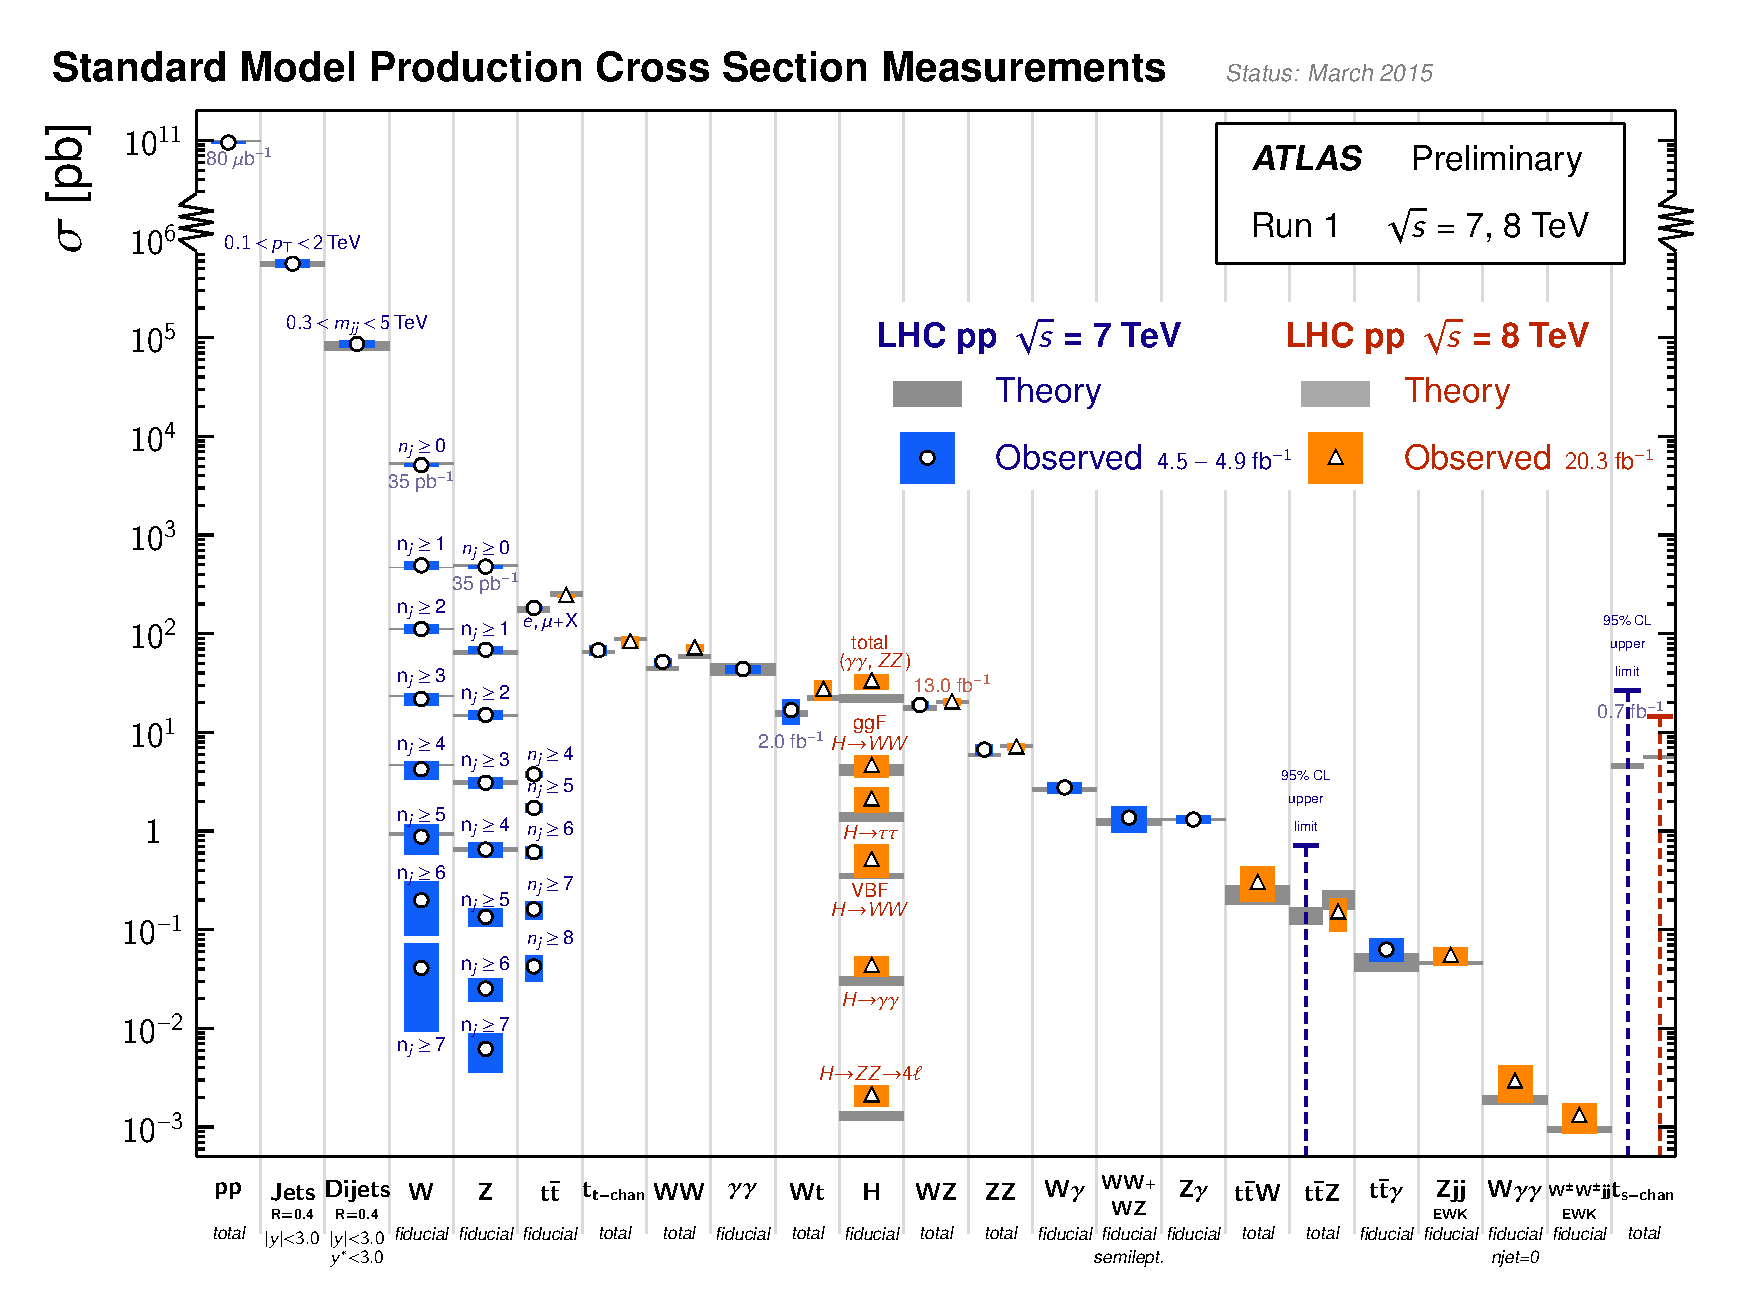
\includegraphics[width=0.7\textwidth]{summary.pdf}
\label{fig:sm:summary}
\caption{Summary of SM cross-section measurements performed in ATLAS, showing the theoretical prediction and the observed value. The agreement across all the various channels is striking.}
\end{figure}

%%%%%%%%%%%%%%%% 

The theory consists of two main parts: the Glashow-Weinberg-Salam theory of electroweak interactions, which describes the electromagnetic and weak nuclear forces, and Quantum Chromodynamics, which describes the strong nuclear force. Together these form the symmetry group of the Standard Model, $SU(3)_C \otimes SU(2)_W \otimes U(1)_Y$. With the discovery of the Higgs Boson, the mechanism of symmetry breaking in the electroweak sector has been elucidated, and all the particles predicted by the model have been identified. While the SM is complete in this sense (, there are still many questions which it does not address, and some of these will be addressed in Chapter~\ref{chapter:susy} and \ref{chapter:search}. At the same time, some predictions of the SM-- the decay channels of the Higgs Boson, or the details of parton showering in QCD-- are still not fully understood, and one new measurement of such SM phenomena is presented in Chapter~\ref{chapter:color}. The following sections give an overview of the SM and outline some of its most powerful successes. The approach will be very cursory, aiming to give a broad overview of the SM Lagrangian and how various parts of it function; detailed references can be found in \ldots. \editnote{Citations on main historial papers?}



\section{The Electroweak Force and Spontaneous Symmetry Breaking}

\editnote{How do I cite Schwartz?}

To start, it is interesting to characterize the electroweak force, i.e. the $SU(2)_W \otimes U(1)_Y$ part of the SM. Note that the $U(1)_Y$ is the gauge group of \textit{hypercharge}, not the low-energy $U(1)$ associated with electromagnetism. Similarly, the particles associated with the $SU(2)_W$ are not the vector bosons $W$ and $Z$: instead, linear combinations of all these fields form the familiar mass eigenstates. 

The Lagrangian of the electroweak sector is:
%
\begin{equation}
\mL = - \frac{1}{4} (W_{\mu\nu}^a)^2 - \frac{1}{4} B_{\mu\nu}^2 + (D_\mu H)^\dagger (D_\mu H) + m^2 H^\dagger H - \lambda(H^\dagger H)^2,
\end{equation}
%,
where $W_\mu^a$ are the $SU(2)$ gauge bosons, $B_\mu$ is the hypercharge gauge boson (and $B_{\mu\nu} = \partial_\mu B_\nu - \partial_\nu B_\mu$), and $H$ is a complex doublet with hypercharge $1/2$, called the Higgs multiplet. The covariant derivative $D_\mu$ is defined as:
%
\begin{equation}
D_\mu H = \partial_\mu H - i g W_\mu^a \tau^a H - \frac{1}{2} i g' B_\mu H,
\end{equation}
%
with $g$ and $g'$ as the $SU(2)$ and $U(1)$ coupling constants, and $\tau^a$ as the standard $SU(2)$ generator. The last part of the Lagrangian, $V(H) = -m^2 |H|^2 +\lambda |H|^4$, is the \textit{Higgs potential}. A potential of this form has a minimum at $|\langle H \rangle| = \sqrt{\frac{2 m^2}{\lambda}}$, which induces a vacuum expectation value (vev) in the potential. This vev breaks the symmetry of the potential. Written out in terms of the multiplet, and taken as real and in one direction only without loss of generality, this vev can be written as:
%
\begin{equation}
H = \exp \left( 2i \frac{\pi^a \tau^a}{v} \right) \colvec{2}{0}{\frac{v}{\sqrt{2}}+ \frac{h}{\sqrt{2}}}
\end{equation}
%
where $v = m / \sqrt{\lambda}$, and $h$ is a real scalar field. The choice of unitary gauge allows us to set $\pi = 0$, simplifying the phase of the vev. Plugging this into the covariant derivative term, and ignoring $h$ terms for now, we have:
%
\begin{equation}
|D_\mu H|^2 = g^2 \frac{v^2}{8} \left[ (W_\mu^1)^2 + (W_\mu^2)^2 + \left( \frac{g'}{g} B_\mu - W_\mu^3 \right) \right]
\end{equation}
%
These are the mass terms of the three massive gauge bosons (each proportional go $\frac{g^2 v^2}{8}$): the breaking of the symmetry of the Higgs potential with the vev has given each of the initially massless bosons a mass. To simplify these masses, we introduce $\tan(\theta_w) = \frac{g'}{g}$, which allows us to write:
%
\begin{align}
Z_\mu &\equiv \cos \theta_w W_\mu^3 - \sin \theta_w B_\mu\\
A_\mu &\equiv \sin \theta_w W_\mu^3 + \cos \theta_w B_\mu
\end{align}
%
and introduce a change of linear basis for the $W^{1,2}$ terms as $W_\mu^{\pm} \equiv \frac{1}{\sqrt{2}} (W_\mu^1 \mp i W_\mu^2)^2$. Plugging this into the original mass terms, we get:
%
\begin{align}
m_A &= 0\\
m_W &= \frac{v}{2} g\\
m_Z &= \frac{v}{2} \sqrt{g^2 +g'^2} = \frac{m_W}{\cos \theta_w}
\end{align}
%
These are the mass terms of the familiar photon, $W$, and $Z$ bosons. Using these transformations on the rest of the original Lagrangian allows for the derivation of the kinetic terms of each boson, as well as the interactions (which are considerably more complicated now that we have broken the original electroweak symmetry).  

Returning now to the previously ignored $h$ term, we can collect its kinetic terms and couplings to get:
%
\begin{equation}
\mathcal{L}_\mathrm{Higgs} = - \frac{1}{2} h \left(\square + \frac{2\lambda}{v^2}\right) h + \mathrm{interactions}.
\end{equation}
%
These are the kinetic and (tree-level) mass terms of a new scalar particle, the Goldstone boson associated with the vev spontaneously breaking the electroweak symmetry. This Higgs boson, discovered by the ATLAS and CMS collaborations on July 4, 2012, was the ``last piece'' of the Standard Model, and its discovery confirmed one of the final open questions of the SM. That is not to say that there are no remaining puzzles, and indeed, Section~\ref{chapter:susy:problems} will address some that are directly related to the Higgs.

\section{Matter}

%define matter fields, how they interact with ew, some lagrangian details, section 29.3 from S

\section{Quantum Chromodynamics and Strong Interactions}

%define QCD lagrangian, discuss renormalization at high level, sign of beta function leading to asymptotic freedom
